\documentclass[12pt, a4paper]{article}
\title{NEA Proposal - IvanChain}
\author{Ivan Leung}
\date{June 2025}


\usepackage[colorlinks=true, linkcolor=black, urlcolor=blue, citecolor=black]{hyperref}
\usepackage[edges]{forest}
\usepackage{graphicx}
\usepackage{float}
\usepackage{fancyhdr}
\usepackage{microtype}
\usepackage[T1]{fontenc}
\usepackage[utf8]{inputenc}
\setlength{\parskip}{\medskipamount}
\setlength{\parindent}{0pt}
\usepackage{babel}
\usepackage{float}
\usepackage{amsmath}
\usepackage{amstext}
\usepackage{varioref}
% \usepackage[unicode=true,pdfusetitle, bookmarks=true,bookmarksnumbered=false,bookmarksopen=false, breaklinks=false,pdfborder={0 0 0},backref=false,colorlinks=false] {hyperref}
\usepackage{setspace}
\usepackage{cleveref}
\usepackage{icomma}
\usepackage{tabu,booktabs}

\graphicspath{{./images/}}
\usepackage{tikz}
\usetikzlibrary{arrows.meta}
\usepackage[scaled]{helvet}
\renewcommand\familydefault{\sfdefault}

\setlength{\parindent}{0pt}
\setlength{\parskip}{1em}

\begin{document}
\fancyhead[L]{Ivan Leung}
\fancyhead[C]{Candidate Number: XXXXXX}
\fancyhead[R]{Centre: 22245}
\fancyfoot[L]{H446}
\fancyfoot[R]{2026}
\pagestyle{fancy}
\maketitle
\newpage
\tableofcontents
\newpage

\section{Analysis}
\label{sec:introduction}

\subsection{The Problem}
Despite many people are investing in cryptocurrency markets, most of them do not understand how blockchain technology (the technology which powers cryptocurrencies) works, 
and there is a lack of educational resources available to help them learn.
The goal is to create a platform where users can learn about blockchain technology, how it works, and how to use it.
\newpage
\subsection{Stakeholders}
People who will be using the system, including developers, users, and administrators.
This also includes the people who would like to invest in cryptocurrencies, allowing them to learn about the technology and how it works.
By understanding the underlying principles of blockchain
\newpage
\subsection{Research}

Blockchain is a distributed ledger technology that allows secure and transparent transactions without the need for a central authority.
This creates a secure, members-only network, ensuring accurate and timely data access. It is often used in technologies such as cryptocurrencies, supply chain management, and digital identity verification.
Blockchains are decentralized, meaning that they are not controlled by a single entity, and they are immutable, meaning that once data is added to the blockchain, it cannot be changed or deleted.
This also means it can only be stored in a peer to peer network, which is a network of computers that are connected to each other and can communicate with each other.


Mining is the process of adding transactions to the blockchain, and it is done by solving complex mathematical problems.
This process is known as Proof of Work (PoW), and it is used to secure the blockchain and prevent double spending.
In PoW, miners compete to solve a mathematical problem, and the first miner to solve the problem gets to add the next block to the blockchain and is rewarded with a certain amount of cryptocurrency.
This process is resource-intensive and requires a lot of computational power, which is why it is often done by specialized hardware known as ASICs (Application-Specific Integrated Circuits). 
This algorithm is used in many cryptocurrencies, such as Bitcoin and Litecoin, to secure the blockchain and prevent double spending.
Proof of Stake (PoS) is an alternative to PoW, where miners are chosen to add the next block to the blockchain based on the amount of cryptocurrency they hold.
This means that the more cryptocurrency a miner holds, the more likely they are to be chosen to add the next block to the blockchain.
This process is less resource-intensive and does not require specialized hardware, making it more accessible to a wider range of users.
This algorithm is used in many newer cryptocurrencies, such as Ethereum 2.0, which is transitioning from PoW to PoS.


\newpage
\subsection{Features}
The platform will have the following features:
\begin{itemize}
    \item Introduction to the platform, allowing users to learn about blockchain technology and how it works.
    \item A graph representation of the users and their relationships, allowing users to see how they are connected to each other.
    \item A visualisation of the blockchain, allowing users to see how the blockchains are connected to each other.
    \item Allowing users to create a new block, add a transaction, and verify a transaction.
    \item Allowing users to transact with each other, to move the blocks around between users.
    \item Checking the blocks in a chain
    \item Checking the users' profiles
    \item Adding users to the system
    \item Settings page allowing users to modify the UI for better aesthetics, such as dark mode
    \item Allow removing users from the system
    \item Allowing users to view the transactions between users
    \item Allowing users to make transactions between users.
\end{itemize}
\newpage
\subsection{Extensions}
The platform can be extended to include more features, such as:
\begin{itemize}
    \item A visualisation of how blocks are created by Proof of Work (PoW), allowing users to see how blocks are added to the blockchain.
    \item Implementing the Proof of Stake (PoS) algorithm, allowing users to see how blocks are added to the blockchain using PoS.
    \item A tutorial system that allows users to learn about controlling the blockchain, such as how to create a new block, how to add a transaction, and how to verify a transaction.
    \item A visualisation of what happens when a blockchain is forked, allowing users to see how the blockchain splits into two separate chains, and how this can be resolved.
    \item Showing different users are mining at the same time and competing to add the next block to the blockchain.
    \item Visualisation on how public and private key pairs play a role in the transaction process, including how they are used to sign transactions and verify ownership.
    \item Introducing multiple chains and visualising the conflict
\end{itemize}
\newpage
    \section{Design}
\subsection{Structure}
\newpage
\subsection{User Interface}

The figure below shows the user interface design of different sections of the platform, including the Introduction Page, Main Page, Users Page, Chains Page, Mining Page, Transactions Page, and the Settings Page.

\begin{figure}[H]
  \centering 
  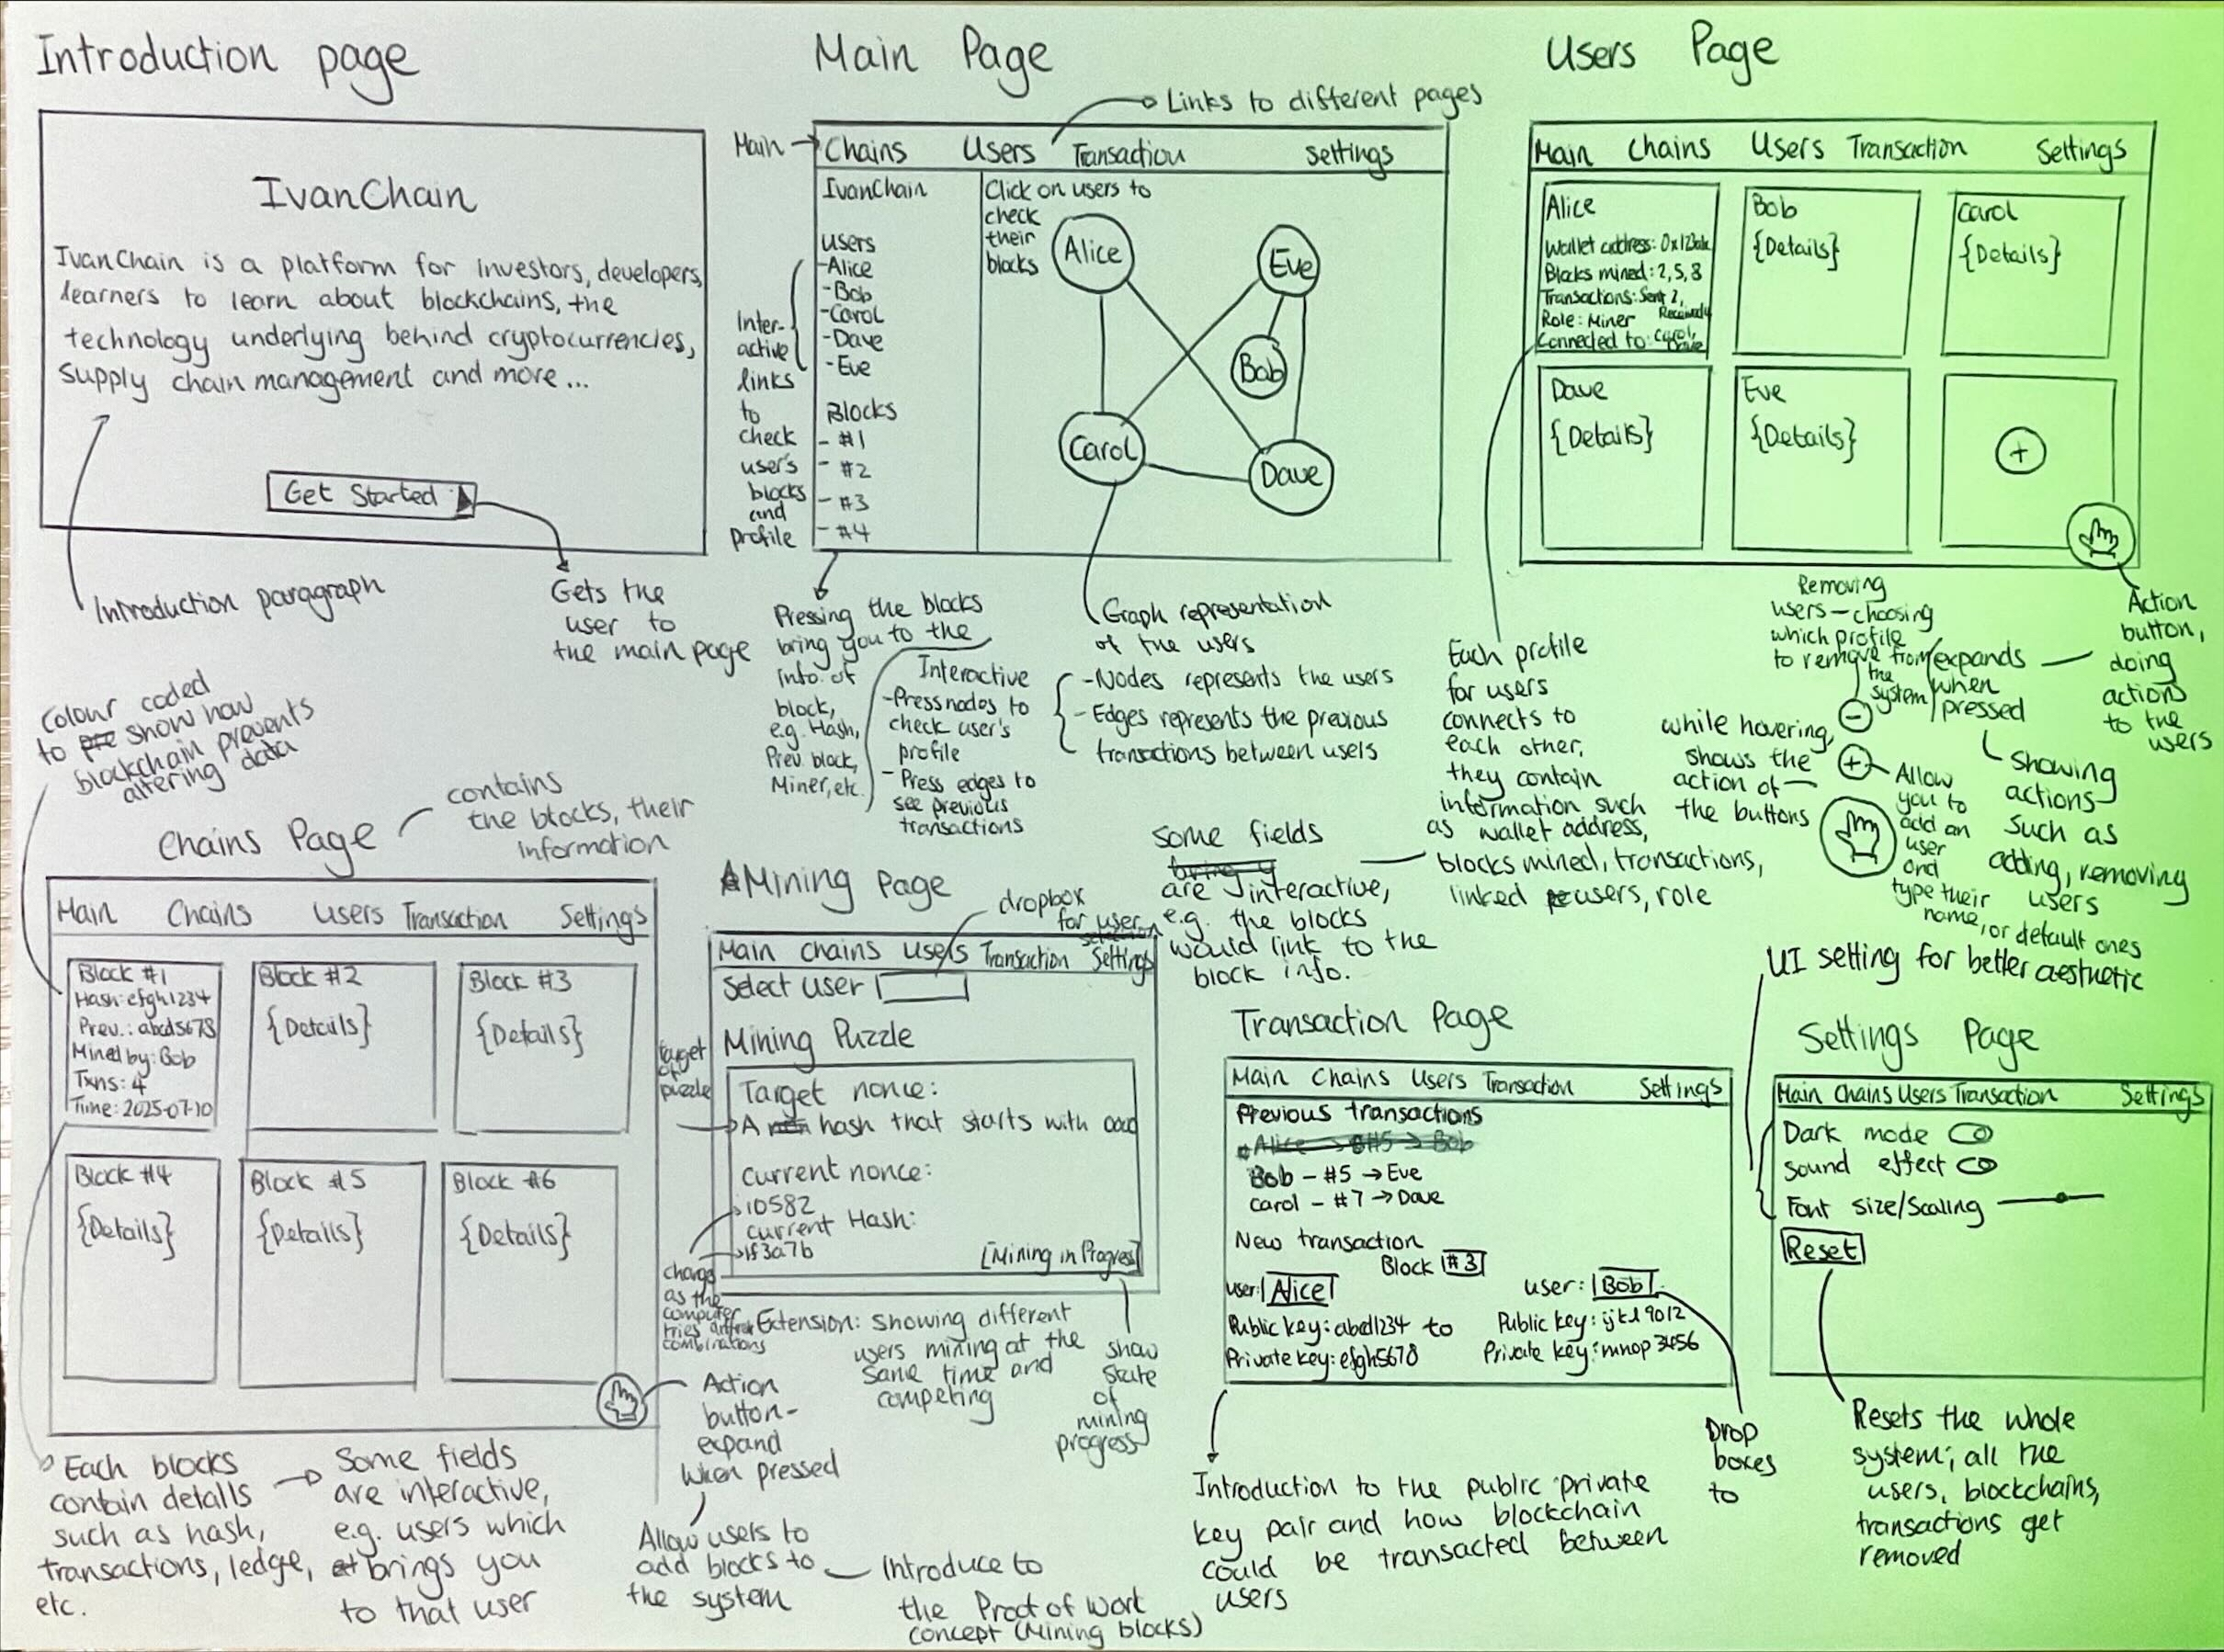
\includegraphics[width=1.2\textwidth]{ui.jpeg}
  \caption{User interface of the blockchain simulator.}
  \label{fig:user-interface}
\end{figure}


\subsection{Decomposition}
\subsection{Algorithms}
\subsection{Test Data}

\section{Development}
\section{Evaluation}
\end{document}